\documentclass[border=3pt,tikz]{standalone}
\usepackage{bm,amsmath}
\usetikzlibrary{patterns,decorations.pathmorphing}
\usetikzlibrary{arrows.meta}
\usetikzlibrary{calc}

% Define the box as a reusable pic component
\tikzset{
  graybox/.pic={
    \coordinate (A) at (0,0);
    \fill[gray!30] (A)--++(\a*\L,0) coordinate (B)--++(\ang:\c*\L) coordinate (C)--++(-0.8*\a*\L,0) coordinate (D)--cycle;
    \draw[gray!50,fill=gray!30,dashed] (C)--++(0,0.8*\b*\L) coordinate (E) --++(-0.8*\a*\L,0) coordinate (F) --(D)--cycle;
    \draw[gray!50,fill=gray!30,dashed] (A)--(D)--(F)--($(A)+(0,\b*\L)$) coordinate (G)--cycle;
    
    \draw[black,fill=gray!30,opacity=0.5] (A)--(B)--($(B)+(0,\b*\L)$) coordinate (H)--(G)--cycle;
    \draw[black,fill=gray!30,opacity=0.5] (B)--(C)--(E)--(H)--cycle;
    \draw[black,fill=gray!30,opacity=0.5] (H)--(E)--(F)--(G)--cycle;
    \node[rotate=0.6*\ang] at ($(B)!0.5!(C)+(0,0.4*\b*\L)$) {$A$};
  }
}

\begin{document}

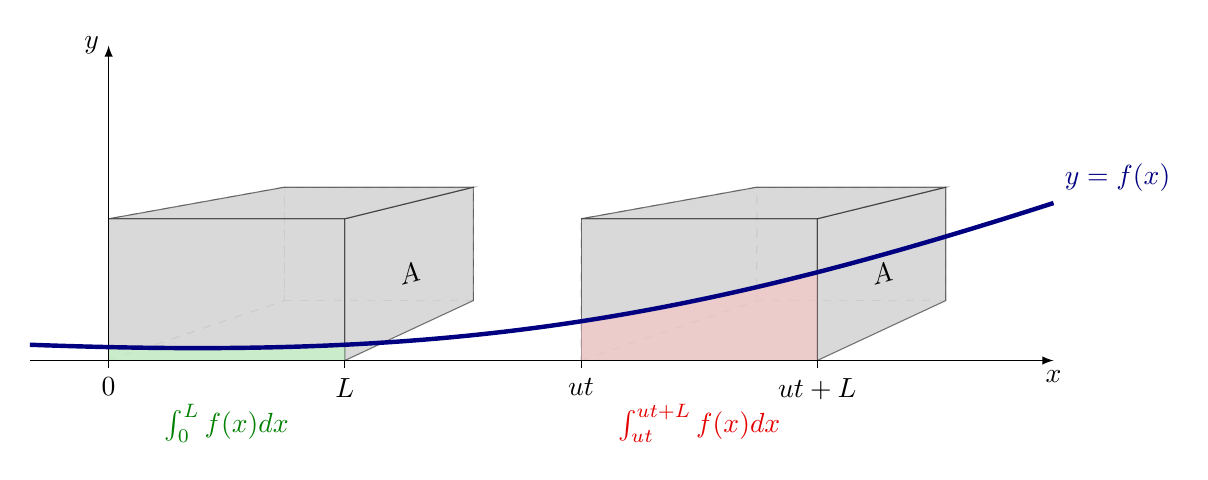
\begin{tikzpicture}

  \def\L{2.0}
  \def\ang{25}
  \def\a{1.5}
  \def\b{0.9}
  \def\c{0.9}
  \def\dL{6}

  % 1. DRAW BOXES FIRST (so they stay in the background)
  \pic at (0,0) {graybox};
  \pic at (\dL,0) {graybox};

  % 2. SHADED AREA (drawn on top of the boxes)
  \begin{scope}
    \clip (0,0) rectangle (\a*\L, \L);
    \fill[green!25,opacity=0.5] (-1,0.1*\L) to[bend right=10] (2*\dL,\L) |- (0,0) -- cycle;
  \end{scope}

  \begin{scope}
    \clip (\dL,0) rectangle (\dL+\a*\L,\L);
    \fill[red!25,opacity=0.5] (-1,0.1*\L) to[bend right=10] (2*\dL,\L) |- (0,0) -- cycle;
  \end{scope}

  
  % 3. AXES
  \draw[-latex] (-1,0)--(2*\dL,0) node[below,pos=1] {$x$};
  \draw[-latex] (0,-0.1)--(0,2*\L) node[left,pos=1] {$y$};
    
  % 4. TICKS AND LABELS
  \draw[dashed] (0,0)--++(0,-0.1) node[below,pos=1] {$0$};
  \draw[dashed] (\a*\L,0)--++(0,-0.1) node[below,pos=1] {$L$};
  \draw[dashed] (\dL,0)--++(0,-0.1) node[below,pos=1] {$ut$};
  \draw[dashed] (\dL+\a*\L,0)--++(0,-0.1) node[below,pos=1] {$ut+L$};
    
  % 5. GREEN CURVE (drawn last so it's fully visible on top)
  \draw[blue!50!black,ultra thick] (-1,0.1*\L) to[bend right=10] node[pos=1, above right] {$y=f(x)$} (2*\dL,\L);

  \node[green!50!black] at (0.5*\a*\L,-0.8) {$\int_{0}^Lf(x)dx$};
  \node[red!90!black] at (\dL+0.5*\a*\L,-0.8) {$\int_{ut}^{ut+L}f(x)dx$};
      
\end{tikzpicture}


\end{document}
